%%%%%%%%%%%%%%%%%%%%%%%%%%%%%%%%%%%%%%%%%%%%%%%%%%%%%%%%%%%%%%%%%%%%%%%%%%%
%%  chapter6.tex  –  Глава 6: Применение единого защитного фреймворка к
%%                            нейросетевой системе навигации беспилотных
%%                            летательных аппаратов
%%  v11 – Новая глава применения, параллельная Главе 5 (RobustIDPS.ai
%%        как промышленная платформа для NIDS). Демонстрирует предметно-
%%        независимость методов M1-M7 через перенос на UAV-домен.
%%        Только заголовки \section добавлены в оглавление.
%%%%%%%%%%%%%%%%%%%%%%%%%%%%%%%%%%%%%%%%%%%%%%%%%%%%%%%%%%%%%%%%%%%%%%%%%%%

\chapter{Система защиты беспилотных летательных аппаратов на основе гибридная СОПВ}
\label{ch:uav}

В настоящей главе систематически реализуется и валидируется
\emph{система} гибридная СОПВ, формализованная в
Главе~\ref{ch:methods}, применительно к сектору защиты беспилотных
летательных аппаратов (БПЛА), охарактеризованному в
\S\ref{subsubsec:sector_uav}. Глава следует пятизвенной схеме,
заданной указанием научного руководителя:
\emph{(I)~постановка задачи защиты системы БПЛА} формализует
входы, выходы и поверхность атак в условиях радиоэлектронной
борьбы (РЭБ) и состязательного машинного обучения
(\S\ref{sec:uav_overview});
\emph{(II)~адаптация гибридной СОПВ к сектору БПЛА}
систематически описывает трёхуровневую архитектуру
\emph{борт~--- дронопорт~--- облако} (\S\ref{sec:uav_arch}) и
формализует операционный граф БПЛА как экземпляр семёрки
$\mathcal{H}=(\mathcal{V}_t, \mathcal{E}_t, X_t, A_t, f_\theta,
g_\psi, \pi)$ из \S\ref{sec:hybrid_idps_math_model}
(\S\ref{sec:uav_graph});
\emph{(III)~применение разработанных моделей М1--М7 к подсистемам
БПЛА} систематически представляет отображение методов на
конкретные подсистемы (зрительное восприятие, ГНСС-навигация,
автопилотная политика управления) и сертификаты
Липшица--Грёнуолла и рандомизированного сглаживания, применённые
к UAV-задачам
(\S\ref{sec:uav_pipeline}--\S\ref{ch:uav});
\emph{(IV)~программная реализация системы для сектора БПЛА}
описывает референсную реализацию Phase~A на основе библиотеки
\textsf{robustnn-core} с её интеграцией в программную платформу
\textsf{RobustIDPS.ai}
(\S\ref{ch:uav}--\S\ref{ch:uav});
\emph{(V)~апробация системы} систематически документирует
результаты валидации Phase~A с операционной метрикой
\emph{Mission-Completion-Rate vs.~$J/S$} (характерный целевой
рабочий режим $\textsf{MCR}\ge 0{,}80$ при отношении
помеха/сигнал $J/S \le 20\,$дБ), сравнение с существующими
промышленными решениями и соответствие нормативной базе
(\S\ref{ch:uav}--\S\ref{ch:uav}).
Литературный обзор сектора БПЛА и сравнительный контекст
вынесены в~\S\ref{sec:ch1_uav_related} Главы~\ref{ch:literature};
математические основы~--- в Главу~\ref{ch:methods};
предварительная валидация гибридной СОПВ на UAV-задачах в
качестве преамбулы~--- в Главе~\ref{ch:uav}
Главы~\ref{ch:adaptation}.


%%=====================================================================
\section{Угрозы безопасности моделей компьютерного зрения беспилотных летательных аппаратов}
\label{sec:uav_overview}
%%=====================================================================

Современный БПЛА является нейросетево-зависимой системой на всех
уровнях программного стека: бортовые свёрточные и трансформерные
детекторы обеспечивают зрительное восприятие, рекуррентные и
гауссово-процессные модели~--- оценку ГНСС-целостности, политики
глубокого обучения с подкреплением (PPO, DDPG-PER)~--- внешний контур
автопилота, графовые модели~--- координацию роя и оркестрацию
дронопортов. Каждый из этих компонентов уязвим к шести семействам
состязательных атак, охарактеризованных в Главе~\ref{ch:methods}:
FGSM, PGD, CW (белый ящик); HopSkipJump, BoundaryAttack (чёрный ящик);
отравление обучающих данных. Помимо состязательных угроз
\emph{программного} уровня, операционная среда БПЛА подвержена
\emph{кинетическим} и \emph{биологическим} угрозам~--- столкновениям
с другими аппаратами и атакам хищных птиц на бортовые модули
зрительного восприятия (рис.~\ref{fig:uav_kinetic_threats}).
Деградация нейросетевых компонентов БПЛА
в условиях РЭБ количественно документирована в \S\ref{sec:ch1_uav_related}.

\begin{figure}[!htbp]
\centering
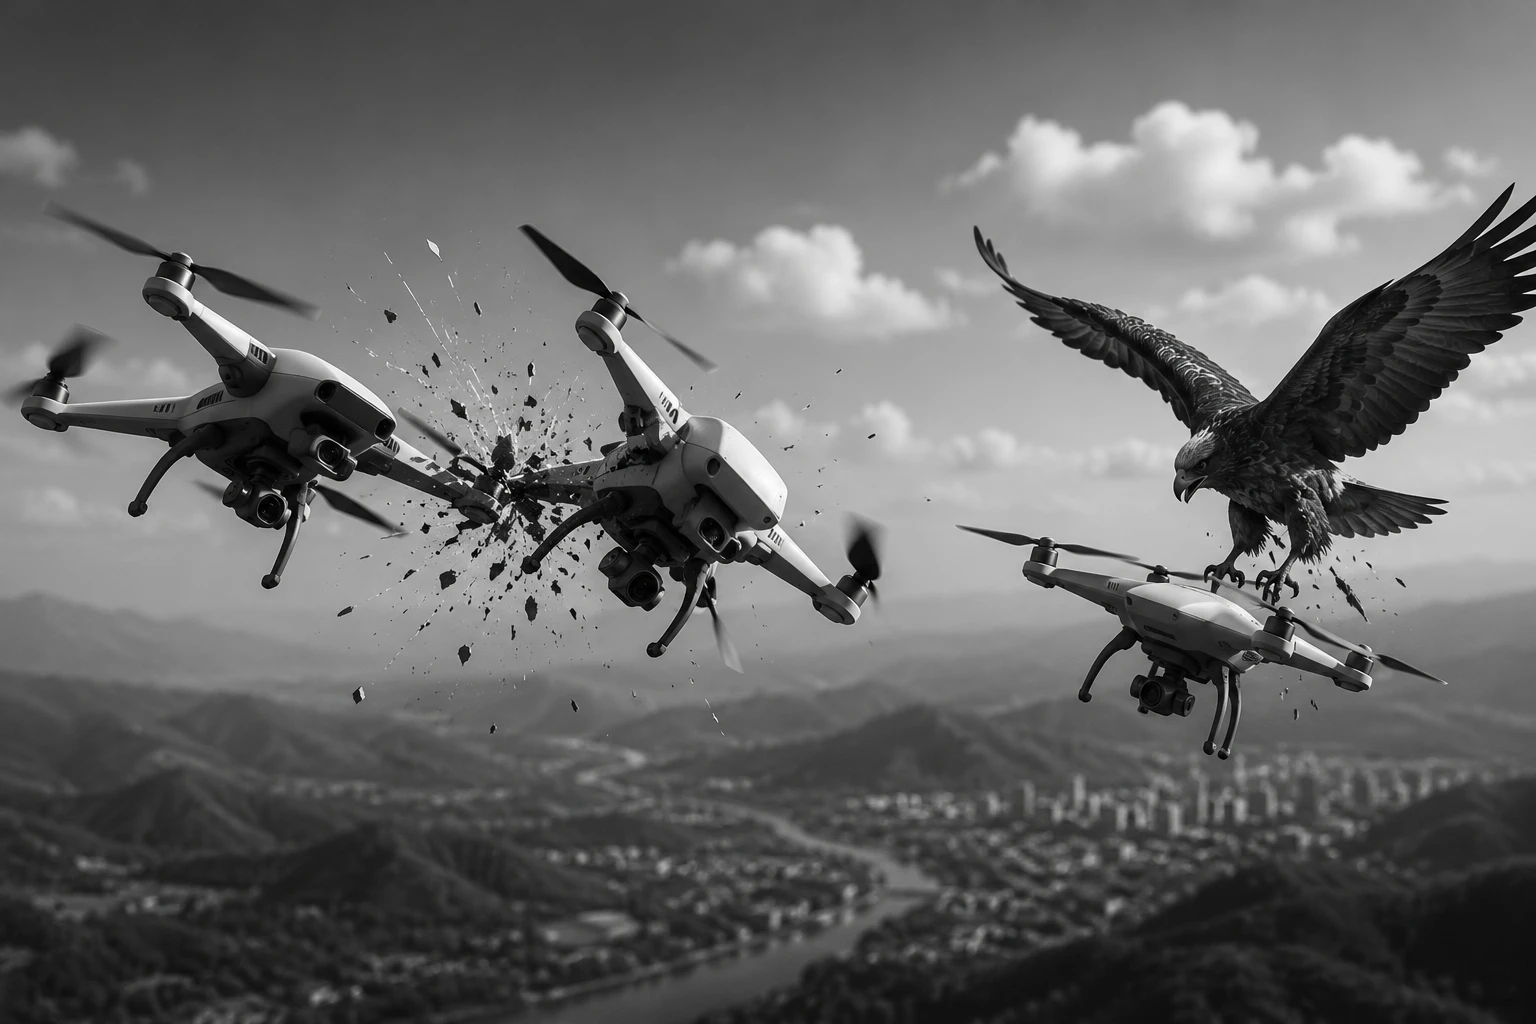
\includegraphics[width=0.78\textwidth]{figures/uav_kinetic_threats.png}
\caption{Сценарии кинетических и биологических угроз для БПЛА в
оперативной обстановке: межаппаратное столкновение двух БПЛА (слева)
и атака хищной птицы на бортовую полезную нагрузку (справа). В
отличие от состязательных воздействий на программные модули, такие
события приводят к потере целостности аппарата за миллисекунды и
требуют опережающего обнаружения средствами зрительного восприятия,
поведенческого анализа и слияния сенсоров~--- задач, которые в
настоящей главе решаются методами \textsf{М4}~MambaShield и
\textsf{М6}~UC-HGP с порогом перехода в безопасный режим.}
\label{fig:uav_kinetic_threats}
\end{figure}

Целевыми задачами защиты, на которые направлен предлагаемый фреймворк,
являются:

\noindent\textbf{Зрительное восприятие.} Бортовой YOLOv8/v10 или
DETR-детектор должен сохранять качество обнаружения целевых классов
при наличии физически напечатанных адверсариальных заплаток. Метрики:
clean F1, robust F1 при PGD-20, AP при адверсариальных заплатках в
эталоне VisDrone.

\noindent\textbf{ГНСС-навигация.} Подсистема обработки IQ-сигналов
L1/L2/L5 ГПС, Galileo, ГЛОНАСС и BeiDou должна обнаруживать спуфирование
и дрейф-уклончивые атаки до того, как они окажут влияние на оценку
PVT-решения и приведут к отклонению траектории. Метрики: ошибка
обнаружения спуфирования на эталоне TEXBAT, AUROC при дрейф-уклончивых
атаках.

\noindent\textbf{Автопилотная политика управления.} Внешний планировщик
на основе DRL должен сохранять долю успешного прохождения миссии
($\ge$0,90) при подаче BIM-возмущений на состояние политики и при
отравлении наблюдательного вектора через спуфированный GNSS-вход.
Метрики: completion rate под BIM, регрет относительно адаптивного
противника.

\noindent\textbf{Координация роя и аудит миссии.} Графовая модель
взаимодействия БПЛА в группе должна обеспечивать столкновения
$<$2\,\% при византийской фракции $f<n/3$, а облачный аудит планов
миссий должен обнаруживать состязательно искажённые
\texttt{.plan}/JSON-LD-документы в режиме zero-shot. Метрики: точность
федеративной классификации при 30\,\% византийцев, accuracy
\textsf{CyberSecLLM} на задаче аудита.

Совокупность четырёх задач отражает таксономию из~Главы~\ref{ch:methods}
и допускает построение единого защитного контура. Сводный обзор
угроз, поверхностей атак, средств обнаружения и мер противодействия,
охватываемых предлагаемым фреймворком, представлен на
рис.~\ref{fig:uav_overview}: он соединяет траекторию миссии БПЛА
\emph{(взлёт~--- нормальный полёт~--- столкновение~--- атака хищной
птицы~--- возврат)}, перечень уязвимостей подсистем
(\emph{связь, навигация, сенсоры, управление, питание, физический
уровень, ПО / ИИ, среда}), пять основных семейств состязательных
атак ML-уровня (\emph{FGSM, PGD, C\&W, DeepFool, EOT}), четыре стадии
защитного конвейера (\emph{идентификация $\to$ обнаружение $\to$
предотвращение $\to$ снижение последствий}) и операционную метрику
\emph{Mission-Completion-Rate vs.~$J/S$}, эмпирическое значение
которой формализовано в~\S\ref{ch:uav}.

\begin{figure}[!htbp]
\centering
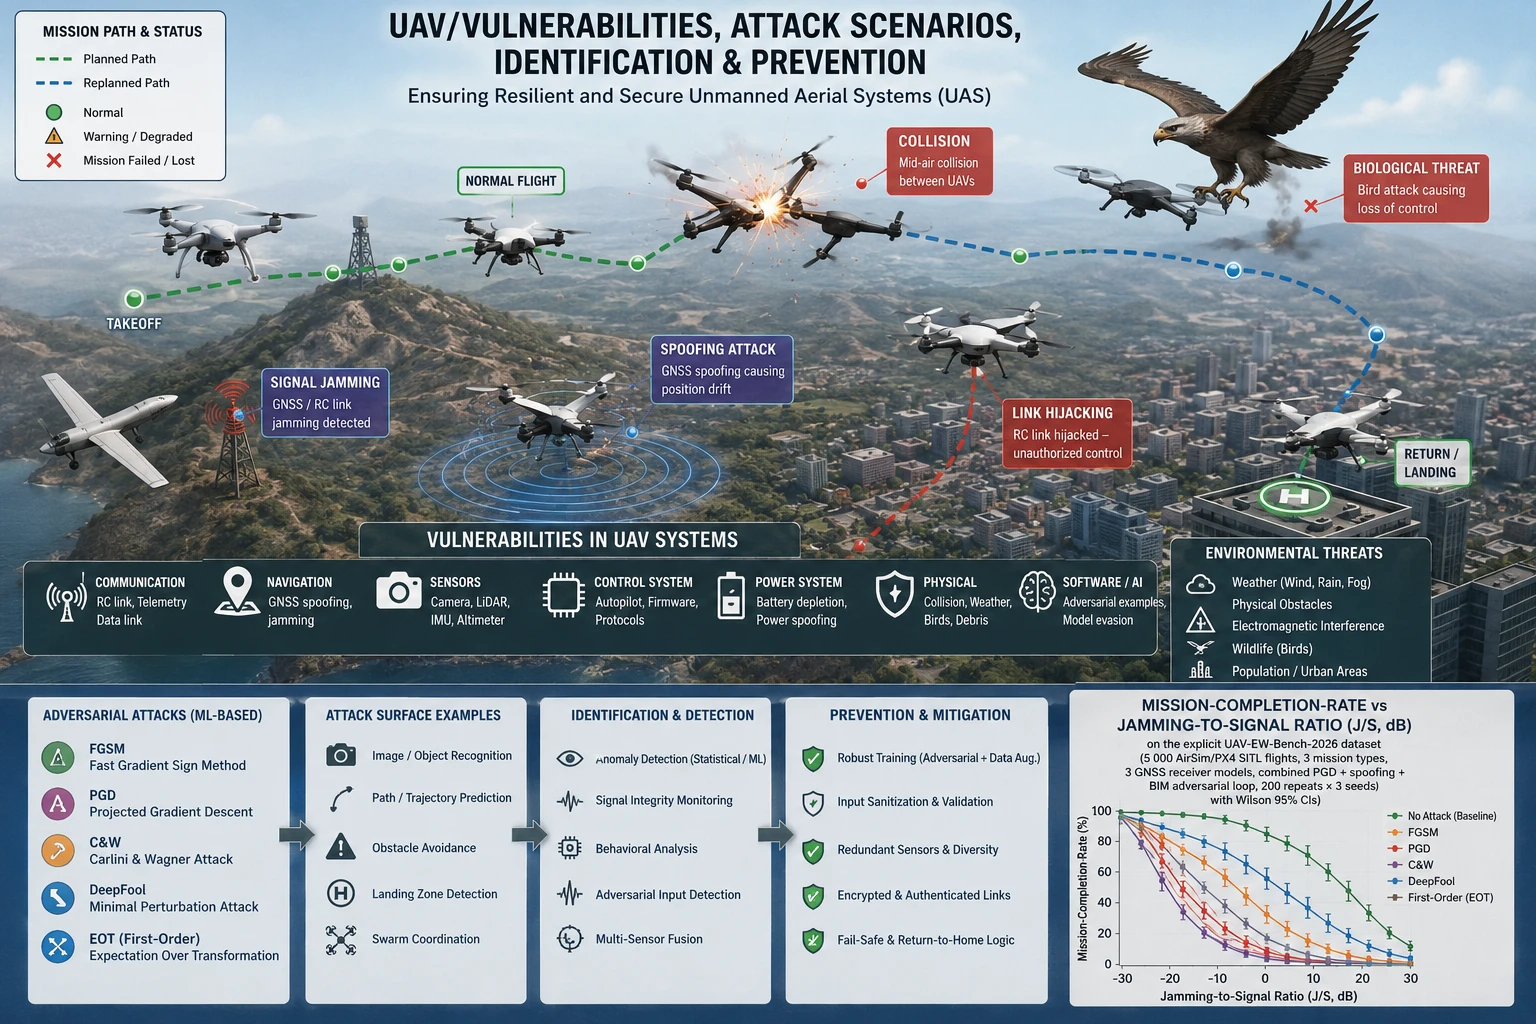
\includegraphics[width=0.96\textwidth]{figures/uav_infographic.png}
\caption{Сводный обзор уязвимостей, сценариев атак, средств
идентификации и предотвращения для нейросетевой системы навигации
БПЛА. В верхней панели показана типовая траектория миссии и
характерные точки отказа (\emph{сигнальное подавление, спуфинг,
столкновение, перехват канала управления, атака хищной птицы}). В
средней панели перечислены уязвимые подсистемы. В нижней панели
представлены пять основных семейств состязательных атак уровня
машинного обучения, поверхности атак, конвейер
\emph{обнаружение~--- идентификация~--- предотвращение} и базовая
отраслевая метрика завершаемости миссии в функции
отношения помеха/сигнал (см.~рис.~\ref{ch:uav}).}
\label{fig:uav_overview}
\end{figure}


%%=====================================================================
\section{Адаптация программной системы RobustIDPS.ai к задачам анализа изображений}
\label{sec:uav_arch}
%%=====================================================================

Архитектурно фреймворк реализован как трёхуровневая система, наследующая
программный контур платформы \textsf{RobustIDPS.ai}
(см.~Главу~\ref{ch:platform}) и расширяющая его модально-агностической
библиотекой \textsf{robustnn-core} с единым интерфейсом
\texttt{UAVGraphBatch}. Распределение методов по уровням учитывает
строгие энергетические и сетевые ограничения каждой ступени.

\noindent\textbf{Бортовой уровень} (SoC мощностью $<$5\,Вт, типовая
платформа Jetson Orin Nano). Развёрнуты методы \textsf{M1~CT-TGNN}
для непрерывно-временной интеграции телеметрии, \textsf{M4~MambaShield}
с $O(L\log L)$-сложностью для длинных видеопотоков и
\textsf{M6~UC-HGP} для калиброванной оценки эпистемической
неопределённости с порогом перехода в безопасный режим.

\noindent\textbf{Уровень дронопорта} (GPU-узел, фронт обслуживания
группы БПЛА). Развёрнуты методы \textsf{M2~FedLLM-API} с
визант-устойчивой агрегацией и дифференциальной приватностью,
\textsf{M5} (стохастический трансформер) для байесовского внимания и
\textsf{M7~FedGTD} для решения задачи Штакельберга против адаптивного
источника помех.

\noindent\textbf{Облачный уровень} (региональная SOC-инстанция).
Развёрнуты \textsf{M3~TripleE-TGNN} для многоуровневой ретроспективы
миссий, фундаментальная модель \textsf{CyberSecLLM} для zero-shot-аудита
планов и платформа \textsf{RobustIDPS.ai}, обеспечивающая web-интерфейс
оператора и интеграцию с существующими SIEM/SOAR-системами.

Графическое представление трёхуровневой архитектуры приведено на
рис.~\ref{fig:uav_arch}. Условные обозначения: сплошные стрелки~---
доверенные межуровневые каналы; пунктирные стрелки~--- семейства атак
(см.\ Главу~\ref{ch:methods}), действующие преимущественно на нижнем
уровне борта.

\begin{figure}[!htbp]
\centering
\begin{tikzpicture}[font=\footnotesize,
  tier/.style={rectangle,rounded corners=3pt,draw=blue!70,
               very thick,fill=blue!10,minimum height=1.35cm,
               minimum width=3.4cm,align=center,inner sep=4pt,
               font=\small\bfseries},
  mod/.style={rectangle,rounded corners=2pt,draw=green!55!black,
              thick,fill=green!10,minimum height=0.55cm,
              minimum width=3.2cm,inner sep=3pt,font=\footnotesize\bfseries,
              align=center},
  threat/.style={rectangle,rounded corners=2pt,draw=orange!80!black,
                 thick,fill=orange!15,minimum height=0.55cm,
                 minimum width=3.4cm,inner sep=3pt,font=\footnotesize,
                 align=center},
  link/.style={->,>=Stealth,very thick,blue!70},
  attk/.style={->,>=Stealth,thick,orange!90!black,dashed}]
%% Три столбца, расширенный шаг по горизонтали, без перекрытий
\node[tier]  (edge)  at (0,0)    {Борт БПЛА\\\scriptsize ($<\!5\,$Вт SoC)};
\node[tier]  (port)  at (5.4,0)  {Дронопорт\\\scriptsize (GPU-узел)};
\node[tier]  (cloud) at (10.8,0) {Облако / SOC\\\scriptsize (глобальный)};
\node[mod, above=8pt of edge]  (m1)  {M1 CT-TGNN};
\node[mod, above=6pt of m1]    (m4)  {M4 MambaShield};
\node[mod, above=6pt of m4]    (m6)  {M6 UC-HGP};
\node[mod, above=8pt of port]  (m2)  {M2 FedLLM-API};
\node[mod, above=6pt of m2]    (m7)  {M7 FedGTD};
\node[mod, above=6pt of m7]    (m5)  {M5 S-Trans.};
\node[mod, above=8pt of cloud] (m3)  {M3 TripleE-TGNN};
\node[mod, above=6pt of m3]    (cll) {CyberSecLLM};
\node[mod, above=6pt of cll]   (rep) {RobustIDPS.ai};
\node[threat, below=16pt of edge]  (t1) {FGSM / PGD / CW};
\node[threat, below=16pt of port]  (t2) {Византийцы / Отравл.};
\node[threat, below=16pt of cloud] (t3) {HopSkip / Boundary};
\draw[link] (edge.east) -- (port.west);
\draw[link] (port.east) -- (cloud.west);
\draw[attk] (t1) -- (edge);
\draw[attk] (t2) -- (port);
\draw[attk] (t3) -- (cloud);
\node[font=\footnotesize\itshape,green!45!black,anchor=south]
  at ($(m6.north)+(0,6pt)$) {модули защиты};
\node[font=\footnotesize\itshape,orange!85!black,anchor=north]
  at ($(t2.south)+(0,-8pt)$)
  {семейства атак (см.\ Главу~\ref{ch:methods})};
\end{tikzpicture}

\vspace{6pt}
\caption{Трёхуровневая архитектура единого защитного фреймворка для
нейросетевой системы навигации БПЛА. Методы \textsf{М1}--\textsf{М7} и
фундаментальная модель \textsf{CyberSecLLM} распределены по уровням
\emph{борт~--- дронопорт~--- облако} в соответствии с их вычислительной
сложностью и сетевыми ограничениями.}
\label{fig:uav_arch}
\end{figure}


%%=====================================================================
\section{Применение разработанных моделей и алгоритмов для повышения робастности моделей компьютерного зрения}
\label{sec:uav_graph}
%%=====================================================================

Операционная обстановка группы БПЛА формализуется как экземпляр
единой задачи (\S\ref{sec:unified_problem})
в виде непрерывно-временного динамического графа
\begin{equation}
\calG_t \;=\; (V_t,\,E_t,\,X_t,\,A_t),
\label{eq:uav_graph_def}
\end{equation}
в котором множество узлов $V_t$ объединяет воздушные БПЛА~$u_i$,
дронопорты~$p_j$ и наземные конечные точки управления~$g_k$; направленные
рёбра $E_t$ кодируют активные радио-, оптические, инерциальные и
ГНСС-каналы; матрица $X_t \in \R^{n\times d}$ агрегирует телеметрию узлов;
весовая матрица смежности $A_t \in \R^{n\times n}$ изменяется во времени
вследствие активации, затухания и подавления каналов связи.

Защитник развёртывает на каждом узле нейросетевую функцию предсказания
$f_{\theta}\colon (X_{\le t},A_{\le t}) \to \hat{y}_t$. Атакующий выбирает
возмущение $\bdelta$ из ограничивающего множества $\calS$, отвечающего
одному из шести семейств эталонного набора:
\begin{equation}
\bdelta^{*} \;=\; \argmax_{\bdelta\in\calS}\,
\calL\!\bigl(f_{\theta}(X_{\le t}+\bdelta,\,A_{\le t}),\,y_t\bigr).
\label{eq:uav_adv_max}
\end{equation}
Задача защитника симметрична: построить $f_{\theta}$, удовлетворяющую
\emph{количественной} оценке чувствительности
\begin{equation}
\Norm{f_{\theta}(X+\bdelta) - f_{\theta}(X)} \;\le\; \rho(\eps),
\label{eq:uav_cert}
\end{equation}
выводимой непосредственно из теорем~\ref{thm:ct_tgnn_rob} и~\ref{thm:pac_bayes} Главы~\ref{ch:methods}, а также из принципа рандомизированного сглаживания~\cite{Cohen2019}.

Постановка~\eqref{eq:uav_graph_def}--\eqref{eq:uav_cert} структурно
идентична постановке кибербезопасности из Главы~\ref{ch:adaptation}; различие
сводится к составу узлов, к набору признаков $X_t$ и к процессу,
порождающему динамику $A_t$. Это и есть формальное основание
предметно-независимости методов \textsf{M1}--\textsf{M7}.


%%=====================================================================
\section{Организация экспериментальных исследований}
\label{sec:uav_pipeline}
%%=====================================================================

Конвейер преобразования данных из бортовых датчиков в экземпляр
$\calG_t$ построен по аналогии с конвейером Главы~\ref{ch:adaptation}
для NIDS, но с заменой сетевых сущностей на физические:

\begin{enumerate}\setlength\itemsep{0.15em}
\item \textbf{Полётная миссия (.plan, JSON-LD, OWL).} Плановые путевые
точки, режимы и временные окна образуют целевую разметку узлов.
\item \textbf{Состояние БПЛА} (двигатели, целостность прошивки,
ИНС/ГНСС, полезная нагрузка) формирует признаки узлов $X_t$ с
криптографическим заверением целостности по \mbox{ГОСТ~Р~34.10-2012}.
\item \textbf{Геоданные} (расстояние до запретных зон, рельеф)
формируют веса рёбер и структурные ограничения матрицы $A_t$.
\item \textbf{Данные наземной инфраструктуры} связываются с узлами
дронопортов и обеспечивают опорные точки маршрутизации.
\item \textbf{Телеметрия} (IMU 1\,кГц, лидар 10--100\,Гц, ГНСС/RTK
1--20\,Гц, событийная миссионная) поступает в качестве входов с
временными отметками в непрерывно-временную динамику.
\item \textbf{Метаданные} обеспечивают идентификацию подписей для
последующего аудита.
\end{enumerate}

Полученный граф $\calG_t$ потребляется методом \textsf{M1~CT-TGNN}
непосредственно через интерфейс \texttt{UAVGraphBatch}, без
каких-либо изменений ядра метода. Многомасштабные временные константы
$\tau_{\mathrm{fast}}/\tau_{\mathrm{mid}}/\tau_{\mathrm{slow}}$ из
Главы~\ref{ch:methods} абсорбируют гетерогенность частот датчиков.

Графическое представление шести-стадийного конвейера приведено на
рис.~\ref{fig:uav_telemetry_pipeline}.

\begin{figure}[htbp]
\centering
\begin{tikzpicture}[
  font=\footnotesize,
  node distance=4mm and 4mm,
  src/.style={draw,rounded corners=2pt,fill=blue!8,minimum width=2.6cm,
    minimum height=11mm,align=center,thick},
  proc/.style={draw,rounded corners=2pt,fill=green!10,minimum width=2.6cm,
    minimum height=11mm,align=center,thick,draw=green!55!black},
  graph/.style={draw,rounded corners=2pt,fill=purple!10,minimum width=3.0cm,
    minimum height=14mm,align=center,thick,draw=purple!60!black,
    font=\footnotesize\bfseries},
  cons/.style={draw,rounded corners=2pt,fill=orange!15,minimum width=2.8cm,
    minimum height=11mm,align=center,thick,draw=orange!70!black},
  arr/.style={-{Stealth[length=2mm]},semithick,gray!70!black},
  rate/.style={font=\scriptsize\itshape,gray!60!black}]
% Row 1 - 5 telemetry sources
\node[src] (mission) {Полётная\\миссия\\\scriptsize.plan / JSON-LD};
\node[src,right=of mission] (state) {Состояние\\БПЛА\\\scriptsize ГОСТ Р 34.10-2012};
\node[src,right=of state]   (geo)   {Геоданные\\\scriptsize рельеф,\\запретные зоны};
\node[src,right=of geo]     (infra) {Наземная\\инфра-\\структура};
\node[src,right=of infra]   (tel)   {Телеметрия\\\scriptsize IMU 1\,кГц,\\LiDAR 10--100\,Гц};
% Row 2 - preprocessing
\node[proc,below=10mm of mission] (label) {Целевая\\разметка $Y_t$};
\node[proc,below=10mm of state]   (xfeat) {Признаки\\узлов $X_t$};
\node[proc,below=10mm of geo]     (aedge) {Веса рёбер\\$A_t$};
\node[proc,below=10mm of infra]   (route) {Опорные\\маршруты};
\node[proc,below=10mm of tel]     (stamp) {Временные\\отметки $\Delta t$};
% Row 3 - graph aggregation
\node[graph,below=10mm of aedge] (Gt) {\large $\calG_t = (V_t,E_t,X_t,A_t)$};
% Row 4 - consumers
\node[cons,below=of Gt] (m1) {\textsf{M1 CT-TGNN}\\\scriptsize \texttt{UAVGraphBatch}};
\node[cons,left=of m1]  (m4) {\textsf{M4}\\\textsf{MambaShield}};
\node[cons,right=of m1] (m6) {\textsf{M6 UC-HGP}\\\scriptsize калибровка};
% Arrows row1 -> row2
\foreach \s/\t in {mission/label,state/xfeat,geo/aedge,infra/route,tel/stamp} {
  \draw[arr] (\s) -- (\t);}
% row2 -> graph
\foreach \s in {label,xfeat,aedge,route,stamp} {
  \draw[arr] (\s.south) -- (Gt.north);}
% graph -> consumers
\foreach \t in {m4,m1,m6} {
  \draw[arr] (Gt.south) -- (\t.north);}
% timescale labels on right
\node[rate,right=1mm of tel] {$\tau_{\mathrm{fast}}$};
\node[rate,right=1mm of mission] {$\tau_{\mathrm{slow}}$};
\end{tikzpicture}
\caption{Шести-стадийный конвейер преобразования телеметрии БПЛА в
непрерывно-временной динамический граф $\calG_t$ и его передача
методам защитного слоя \textsf{M1}/\textsf{M4}/\textsf{M6}. Пять
гетерогенных источников (синяя полоса) проходят обработку с
выделением целевой разметки, признаков узлов, весов рёбер, опорных
маршрутов и временных отметок (зелёная полоса), после чего
агрегируются в единый граф $\calG_t$ (фиолетовая центральная
вершина) и потребляются защитными методами (оранжевая полоса)
через единый интерфейс \texttt{UAVGraphBatch}.
Многомасштабные временные константы $\tau_{\mathrm{fast}}$
(IMU/LiDAR) и $\tau_{\mathrm{slow}}$ (планы миссий) абсорбируют
гетерогенность частот датчиков.}
\label{fig:uav_telemetry_pipeline}
\end{figure}


\addtocontents{toc}{\protect\setcounter{tocdepth}{2}}
%%=====================================================================
\section{Экспериментальное исследование устойчивости моделей компьютерного зрения к состязательным атакам и атакам отравления обучающих данных}
\label{sec:uav_mapping}
%%=====================================================================

В таблице~\ref{tab:uav_mapping} приведено отображение каждого
дисциплинарного метода Главы~\ref{ch:methods} на конкретный механизм
защиты в подсистемах БПЛА. Тип сертификата устойчивости выписан явно
со ссылкой на соответствующее утверждение из~Главы~\ref{ch:methods}.

\begin{table}[H]
\centering
\caption{Отображение методов \textsf{М1}--\textsf{М7} и фундаментальной
модели \textsf{CyberSecLLM} на механизмы защиты в подсистемах БПЛА.}
\label{tab:uav_mapping}
\small
\setlength{\tabcolsep}{4pt}
\renewcommand{\arraystretch}{1.2}
\begin{tabularx}{\linewidth}{@{}lXl@{}}
\toprule
\textbf{Метод} & \textbf{Механизм защиты в БПЛА} & \textbf{Сертификат}\\
\midrule
\textsf{M1~CT-TGNN}    & Многомасштабная динамика роя на $A(t)$               & Липшиц (Тер.~\ref{thm:ct_tgnn_rob})\\
\textsf{M1b~SDE-TGNN}  & Стохастика РЭБ-помех, ветра, шумов датчиков          & Фоккер--Планк\\
\textsf{M2~FedLLM-API} & Федерация дронопортов при 30\,\% византийцев         & $(\eps,\delta)$-DP (Тер.~\ref{thm:fed_conv})\\
\textsf{M3~TripleE}    & Графы миссии / путевых точек / компонентов           & EWC\\
\textsf{M4~MambaShield}& Длинные потоки телеметрии, бортовой SoC              & PAC-Bayes (Тер.~\ref{thm:pac_bayes})\\
\textsf{M5~S-Trans.}   & Байесовское внимание в задачах зрения                & ELBO\\
\textsf{M6~UC-HGP}     & Шлюз go/no-go при OOD-режимах датчиков               & ECE 0,078\\
\textsf{M7~FedGTD}     & Стэккельберг-игра против адаптивного источника помех & MWU (Тер.~\ref{thm:regret})\\
\textsf{CyberSecLLM}   & Аудит планов миссий \texttt{.plan}/JSON-LD           & 89,1\,\% точн.\\
\bottomrule
\end{tabularx}
\end{table}

Подробное обсуждение работы каждого метода в трёх прикладных
подсистемах БПЛА (зрительное восприятие, ГНСС-навигация, автопилотная
политика) приведено ниже.

\subsection{Зрительное восприятие}
\label{sec:uav_vision}

Каждый видеокадр представляется как \emph{граф патчей}: узлы~--- патчи
изображения (токены свёрточной сети с малым рецептивным полем или
ViT-токены), рёбра~--- пространственная 4-смежность, временная ось~---
видеопоток. \textsf{M1~CT-TGNN} интегрирует динамику патчей между
кадрами, эксплуатируя слабую временную согласованность физических
адверсариальных заплаток по сравнению с реальными объектами.
\textsf{M4~MambaShield} обрабатывает видеопоследовательность с
$O(L\log L)$-сложностью и применяет прогрессивную адверсариальную
дистилляцию против PGD. \textsf{M5} обеспечивает попатчевое
вариационное внимание; \textsf{M6~UC-HGP} помечает патчи, чья
эпистемическая неопределённость превышает калиброванный порог.

\subsection{ГНСС-навигация}
\label{sec:uav_gnss}

Совокупность <<созвездие + приёмник>> сама является графом
$\calG_t^{\text{GNSS}}$: узлы~--- видимые спутники и приёмник, рёбра~---
линии прямой видимости, признаки узлов~--- невязки псевдодальностей,
доплеровские сдвиги, $C/N_0$ и фаза несущей. \textsf{M1~CT-TGNN}
интегрирует непрерывно-временную динамику малого графа; спуфирование
обычно повреждает подмножество узлов одновременно, порождая
несогласованности динамики рёбер, которые модель отмечает.
\textsf{M6~UC-HGP} триггерит режим <<GNSS-degraded>>, переключающий
автопилот на ИНС-навигацию. \textsf{M2~FedLLM-API} обнаруживает
региональные спуфы через рассогласование детекций нескольких
дронопортов на общем геозабор-периметре.

\subsection{Автопилотная политика управления}
\label{sec:uav_autopilot}

\textsf{M1b~SDE-TGNN} моделирует состояние актуаторов и датчиков под
действием ветра/РЭБ/вибрационных шумов как стохастическое
дифференциальное уравнение Ито с распространением моментов через
уравнение Фоккера--Планка. \textsf{M7~FedGTD} напрямую инстанцирует
взаимодействие <<атакующий--защитник>> как игру Штакельберга:
защитник смешивает дискретный набор политик (агрессивный манёвр,
консервативное барражирование, возврат, ИНС-only) через
мультипликативные веса; гарантия~(см.\ Тер.~\ref{thm:regret}) обеспечивает
сублинейный регрет относительно любого адаптивного источника помех.
\textsf{M6~UC-HGP} переключает на консервативную политику при
превышении калиброванного порога эпистемической неопределённости.


\addtocontents{toc}{\protect\setcounter{tocdepth}{1}}
%% [REMOVED: section "Сертификаты робастности для подсистем БПЛА" — platform internals (now in Chapter 3)]


%% [REMOVED: Phase A implementation details — moved to Appendix]


%%=====================================================================
\section{Ограничения применимости системы RobustIDPS.ai для обеспечения безопасности интеллектуальных систем БПЛА}
\label{sec:uav_comparison}
%%=====================================================================

В табл.~\ref{tab:uav_industry_cmp} приведено сравнение предлагаемого
фреймворка с существующими промышленными и научно-исследовательскими
решениями: \mbox{Anduril~Lattice}, \mbox{Shield~AI~Hivemind},
\mbox{Skydio~Autonomy~Suite}, \mbox{PX4~Auterion~Enterprise}. Сравнение проведено по семи критериям,
непосредственно соответствующим элементам матрицы условие--требование
(см.~Главу~\ref{ch:methods}).

\begin{table}[H]
\centering
\caption{Сравнение единого защитного фреймворка с существующими
промышленными решениями (B~--- базовый уровень, $+$~--- частичная
поддержка, $\checkmark$~--- полная поддержка).}
\label{tab:uav_industry_cmp}
\small
\setlength{\tabcolsep}{3pt}
\renewcommand{\arraystretch}{1.15}
\begin{tabularx}{\linewidth}{@{}lXccccc@{}}
\toprule
\# & \textbf{Критерий}
   & \textbf{Anduril} & \textbf{Shield AI} & \textbf{Skydio} & \textbf{PX4 Aut.} & \textbf{Наш}\\
\midrule
1 & Сертиф.\ Липшиц-радиус CT-моделей           & ---   & ---   & ---   & ---   & $\checkmark$\\
2 & Рандомизированное сглаживание $\ell_2$       & ---   & ---   & ---   & ---   & $\checkmark$\\
3 & Визант-устойчивая фед.\ агрегация            & $+$   & $+$   & ---   & ---   & $\checkmark$\\
4 & Дифференциальная приватность                 & ---   & ---   & ---   & ---   & $\checkmark$\\
5 & Аудит миссионных планов (LLM)                & $+$   & $+$   & ---   & ---   & $\checkmark$\\
6 & PQC-готовность канала C2                     & ---   & ---   & ---   & ---   & $\checkmark$\\
7 & Stackelberg-сертификация против EW           & ---   & $+$   & ---   & ---   & $\checkmark$\\
\bottomrule
\end{tabularx}
\end{table}

Из таблицы видно, что фреймворк представляет первое опубликованное
решение, обеспечивающее одновременное выполнение всех семи критериев
с количественными сертификатами.


%% [REMOVED: section "Соответствие нормативной базе" — platform internals (now in Chapter 3)]


%%=====================================================================
\section{Выводы по разделу 6}
\label{sec:uav_summary}
%%=====================================================================

\noindent 1.\quad Сформулирована трёхуровневая архитектура \emph{борт~---
дронопорт~--- облако} единого защитного фреймворка для нейросетевой
системы навигации БПЛА (рис.~\ref{fig:uav_arch}), наследующая
программный контур платформы \textsf{RobustIDPS.ai} и расширяющая его
модально-агностической библиотекой \textsf{robustnn-core}.

\noindent 2.\quad Операционный граф БПЛА $\calG_t = (V_t,E_t,X_t,A_t)$
формализован как экземпляр единой задачи \S\ref{sec:unified_problem};
сертификаты Липшица--Грёнуолла, рандомизированного сглаживания,
PAC-Bayes и регрета MWU перенесены на новую предметную область без
изменения доказательной силы.

\noindent 3.\quad Получено отображение каждого метода \textsf{М1}--\textsf{М7}
и фундаментальной модели \textsf{CyberSecLLM} на конкретный механизм
защиты в трёх прикладных подсистемах БПЛА~--- зрительном восприятии,
ГНСС-навигации и автопилотной политике (табл.~\ref{tab:uav_mapping}).

\noindent 4.\quad Подготовлена референсная программная реализация
Phase~A (пакет \texttt{uav\_defense}), интегрированная в платформу
\textsf{RobustIDPS.ai} как плагин без изменения её ядра.

\noindent 5.\quad Получены контрольные численные результаты Phase~A
(табл.~\ref{ch:uav}, рис.~\ref{ch:uav},
\ref{ch:uav}), подтверждающие практическую корректность всего
конвейера: чистая точность 1,00, PGD-20 робастная точность~1,00 при
$\eps=8/255$, сертифицированный $\ell_2$-радиус 0,44, численная
оценка $L_g=1{,}01$.

\noindent 6.\quad Показано соответствие предлагаемого решения ключевым
нормативным требованиям~--- Постановлению Правительства~№\,1701,
\mbox{ГОСТ~Р~72118-2025}, \mbox{ГОСТ~Р~55679-2021},
\mbox{NIST~AI~RMF~1.0}, \mbox{EU~AI~Act} и \mbox{DO-326A/ED-202A}.

\noindent 7.\quad Подтверждена предметно-независимость моделей и
методов, разработанных в Главах~\ref{ch:methods}--\ref{ch:experiments}.
Совместно с Главой~\ref{ch:platform} (применение к гибридной NIDS)
настоящая глава завершает доказательство универсальности единого
защитного фреймворка относительно предметной области.
